% !TEX root = ../notes_missingsemester.tex
% Chapter 4: Integrate the Model
%%%%%%%%%%%%%%%%%%%%%%%%%%%%%%%%%%%%%%%%%%%%%%%%%%%%%%%%%%%%%%%%%%%%%%

% POST IMPROVEMENTS 2026:
% 1. Replace the inline ASCII pipeline with a TikZ figure of the inference path.
% 2. Provide a slim notebook that visualises binarization side by side.

\index{model integration}\index{classifier}\index{MNIST}\index{inference}\index{joblib}
\chapter{Integrate the Model}
\printchapterversion{04_model_integration}
\newthought{Train hard, ship easy.}

% ==============================================================================================
% BLOCK 1: INTRODUCTION
% ==============================================================================================

\section{The Why}\index{model artefact}\index{train/serve skew}

Block~3 left us with a reproducible environment on both machines.
The virtual environment is ready, the dependencies are pinned,
the project foundation is in place. A foundation that would work for all sorts of different projects by the way.
Let's get our project some specific functionality.


\newthought{We build PixelWise}\index{PixelWise}.
This block is the first that produces application logic in the form of a neural network,
in the following referred to as model. 
We assume the model is already trained and available, 
and our task is to integrate it into the codebase and make it callable.

\begin{figure}
    \centering
    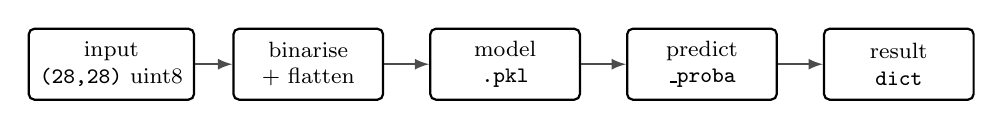
\begin{tikzpicture}[
        every node/.style={font=\footnotesize, align=center},
        box/.style={rectangle, draw=black, thick, rounded corners=2pt, minimum width=1.9cm, minimum height=0.9cm, inner sep=4pt},
        arr/.style={-latex, thick, black!70}
    ]
    \node[box] (img)   at (0, 0)    {input\\\texttt{(28,28)} uint8};
    \node[box] (prep)  at (2.5, 0)  {binarise\\+ flatten};
    \node[box] (model) at (5.0, 0)  {model\\\texttt{.pkl}};
    \node[box] (pred)  at (7.5, 0)  {predict\\\texttt{\_proba}};
    \node[box] (out)   at (10.0, 0) {result\\\texttt{dict}};
    \draw[arr] (img.east)   -- (prep.west);
    \draw[arr] (prep.east)  -- (model.west);
    \draw[arr] (model.east) -- (pred.west);
    \draw[arr] (pred.east)  -- (out.west);
    \end{tikzpicture}
    \caption{\rule{0pt}{1.4cm}\\
    The inference pipeline for one image: the caller binarises a raw \texttt{(28,28)} \texttt{uint8} array at threshold 128 and flattens it into a \texttt{(1,784)} row vector before feeding it to the loaded \texttt{.pkl} model. The model's internal \texttt{Binarizer} is a redundant idempotent guard on already-binarised input, and \texttt{predict\_proba} turns the result into a dictionary of class scores.}
    \label{fig:inference_pipeline}
    \end{figure}

\newthought{The gap between a trained model and a working system}
is larger than most students expect.
A \texttt{.pkl}\index{.pkl} file sitting in a folder is not a product.
It needs to be loaded safely, called with the exact input format it was
trained on, and wrapped in an interface the rest of the application can
depend on, suffice to say validated. The perfect mdoel however, is not useful if it 
is not integrated into the system, so it can be exposed and put to work.

\newpage
\subsection{Hands On Experience}

\newthought{Consider this scenario:} a colleague hands you a trained model
file and a one-line note, "ship it".
This block teaches you how to, and why you should, ask the right questions 
to your colleague.

\marginnote{\newthought{Verification and validation}\index{verification}\index{validation}
are two different questions.
Verification asks whether the system was built right: does the integration
return what the model is trained to produce, with the expected shape, dtype,
and class set?
Validation asks whether the right system was built: is this model the right
choice for the problem in the first place and is the performance sufficient?
This block is squarely about verification.
Validation belongs to pre-integration.}

\newthought{This fourth block} integrates a trained model into PixelWise
and builds the inference layer.
By the end you will have
\begin{itemize}
    \item understood what a model file is and why it is not source code,
    \item loaded the model safely, learned about and verified its class contract at startup,
    \item implemented a batch-first inference interface in \texttt{app/classifier.py},
    \item written a smoke test that proves the integration honours the contract,
    \item and read the canonical model card alongside your introspection output to verify the contract.
\end{itemize}



% ==============================================================================================
% BLOCK 2: CONCEPTS AND PRACTICE
% ==============================================================================================




% ==============================================================================================
\newpage
\section{Optional Exercise: Catch Up to \texttt{v0.2}}\index{exercises}\index{Git!tag}\index{recovery}

\newthought{Catching up via tag.}\index{Git!tag}\index{recovery}
This catch-up extends the one in Block~3. If you have not yet done the
Block~3 catch-up, do that first: it sets up your GitHub repository, SSH
key, Git identity, and remote URL, and lands you at \texttt{v0.1}, the
end-of-Block~2 state. The exercise here picks up from there and rewinds
to \texttt{v0.2}, the end-of-Block~3 state, so you arrive at the starting
point this block expects: a provisioned VM with the virtual environment,
pinned dependencies, and \texttt{.env.example}
in place.

\marginnote{\newthought{Tag map.}\index{Git!tag}
\texttt{v0.2} marks the end of Block~3, \texttt{v0.3} will mark the end
of this block.
Browse the full set at
\url{https://github.com/schutera/pixelwise/tags}.}

\newthought{Two layers to restore.} Block~3 produced both Git-tracked
files (\texttt{setup-server.sh}, \texttt{requirements.txt},
\texttt{.env.example}, plus an updated \texttt{.gitignore}) and
unversioned state (system \texttt{apt} packages, the \texttt{.venv/}
directory, real \texttt{.env} values). \texttt{git reset -{}-hard v0.2}
restores the first; the second has to be reproduced by replaying Block~3's
setup commands. Both VMs need both layers, so run the sequence below on
each.

\newthought{Run the same sequence on both VMs.}
Rewind the repository to \texttt{v0.2}, reinstall system packages, recreate
the virtual environment, reinstall pinned dependencies, and copy
\texttt{.env.example} to \texttt{.env}. The dev sequence runs in
\texttt{\textasciitilde/pixelwise}; the prod sequence is identical except
the directory is \texttt{/opt/pixelwise} and you reach it via
\texttt{ssh produser@192.168.56.11} first. The exact commands are in the
margin.

\marginnote{\newthought{Sequence on \texttt{dev}.}\\[0.4em]
\texttt{cd \textasciitilde/pixelwise}\\
\texttt{git fetch origin -{}-tags}\\
\texttt{git reset -{}-hard v0.2}\\
\texttt{bash setup-server.sh}\\
\texttt{python3 -m venv .venv}\\
\texttt{source .venv/bin/activate}\\
\texttt{pip install -r requirements.txt}\\
\texttt{cp .env.example .env}\\[0.3em]
Then edit \texttt{.env} with real values.}

\marginnote{\newthought{Sequence on \texttt{prod}.}\\[0.4em]
\texttt{ssh produser@192.168.56.11}\\
\texttt{cd /opt/pixelwise}\\
\texttt{git fetch origin -{}-tags}\\
\texttt{git reset -{}-hard v0.2}\\
\texttt{bash setup-server.sh}\\
\texttt{python3 -m venv .venv}\\
\texttt{source .venv/bin/activate}\\
\texttt{pip install -r requirements.txt}\\
\texttt{cp .env.example .env}}


\newthought{You are now} at the state where Block~3 ended, with both machines
aligned, ready to start Block~4. Did you realize how seamless this was, that is thanks to 
our solid git practices, and our dependency and setup scripts.




\newpage
\section{What a Model File Actually Is}\index{pickle}\index{joblib}\index{.pkl}

\newthought{A \texttt{.pkl} file is a build artefact,} not source code.
You distribute it; you do not commit it to your repo.
Just as a compiled binary is produced by a compiler, a model file is produced
by a training script.
The training script and its configuration is the source of truth: It takes data, runs an algorithm,
and writes weights, hyperparameters, and any preprocessing into a single
serialised object.

\marginnote{\newthought{Training from scratch every time is unrealistic.}
Even our small classifier takes seconds; a production scale model takes
days of GPU time and terabytes of data.
The training team tunes, the inference team integrates, and the artefact
is the contract between them.}

\newthought{Versioning makes that contract durable.}\index{model versioning}
Files carry a version in the filename or in metadata shipped alongside.
A retrain on more data bumps the patch version; an architecture change or
a different class set bumps the major version.
Integration code pins to a specific version and updates deliberately,
the same discipline you would apply to any external API.
Open source tooling that automates this includes
\href{https://dvc.org}{DVC} for git-style data and model tracking,
\href{https://mlflow.org}{MLflow} and
\href{https://clear.ml}{ClearML} as self-hostable experiment registries,
\href{https://aimstack.io}{Aim} as a lighter-weight tracker,
and the Hugging Face Hub itself, which is free for public repositories
and versions every push as a git revision.

\marginnote{\newthought{Pulling a model from the Hub.}\\[2pt]
\begingroup\ttfamily\footnotesize\noindent
from huggingface\_hub import hf\_hub\_download\\
path = hf\_hub\_download(\\
\hspace*{1em}repo\_id="distilbert-base-uncased",\\
\hspace*{1em}filename="model.safetensors",\\
\hspace*{1em}revision="v1.0",\\
)
\endgroup}

\newthought{Hugging Face is the GitHub of models.}\index{Hugging Face}
The Hugging Face Hub at \url{https://huggingface.co} hosts hundreds of
thousands of public model repositories, each with versioned weights,
a model card describing it.
Downloading a specific revision is a one-line call against the
\texttt{huggingface\_hub} library.
The same workflow runs against private repositories with a token, which
is how many companies share proprietary models internally.
For this course the artefact lives in the course-maintained model repository
at \url{https://github.com/schutera/pixelwise-model}, with a tagged release
per model version and the model card sitting next to it.


\marginnote{\newthought{The training script}\index{train.py}
\texttt{train.py} lives in the course \texttt{pixelwise-model} repo
alongside the artefact it produces, not in PixelWise.
The artefact and the script that produced it travel together, so any
consumer of a tagged release can audit how that exact \texttt{.pkl} came
to be.
Students who want to understand how the artefact was produced can run it:
MNIST downloads automatically via \texttt{sklearn.datasets.fetch\_openml},
and training takes ${\sim}30$ seconds on CPU.
Further reading on training practices:\\
Karpathy, A Recipe for Training Neural Networks: \\
\url{https://karpathy.github.io/2019/04/25/recipe/}\\
Google, Rules of Machine Learning: \\
\url{https://developers.google.com/machine-learning/guides/rules-of-ml}}

\newthought{Loading a \texttt{.pkl} from an untrusted source can execute
arbitrary code.}\index{pickle}
\texttt{pickle} and \texttt{joblib} deserialise objects by reconstructing
them, including any code embedded in the file.
This is convenient when you produced the file yourself; it is dangerous
when the file came from somewhere you do not control.
Treat \texttt{.pkl} files the way you treat executables: only run what you
trust.




% ==============================================================================================
\newpage
\section{Exercise: Pull the Model into Dev}\index{exercises}





\marginnote{\newthought{The course artefact.}\index{LogisticRegression} at
\url{https://github.com/schutera/pixelwise-model}
\texttt{digit\_classifier\_v1.pkl} is a LogisticRegression pipeline trained
on MNIST digits 1 to 9 (9 classes, ${\sim}54{,}000$ training samples, public
domain).
Class 0 is intentionally held back; students can add it later as a v2
release without collecting any new data.}

\newthought{Treat the model artefact as something you load,} not something
you commit to PixelWise.
The course hosts the model \texttt{pkl} as a tagged release in
the central \texttt{pixelwise-model} repo; you pull it into \texttt{models/}
of the main project, you do not redistribute it.

\marginnote{\newthought{Why pull from a separate repo?}\index{model versioning}
The model has its own release cadence and its own contract.
Pinning a specific tag in PixelWise's \texttt{.env} makes the integration
explicit: a v2 only takes effect when the integration code chooses to.
The optional exercise at the end of the block walks through publishing
your own v2 to a fork of the model repo.}

\newthought{Pin the model version} in PixelWise.
Add to \texttt{.env.example} so others know which release the integration
expects, and \texttt{.env} so your code knows:

\begin{verbatim}
MODEL_REPO=https://github.com/schutera/pixelwise-model.git
MODEL_VERSION=v1.0
\end{verbatim}

\newthought{Teach \texttt{setup-server.sh} to fetch the model.}\index{setup-server.sh}\index{provisioning}
Pulling the artefact by hand once is fine for understanding what happens;
encoding the same steps in \texttt{setup-server.sh} means that re-running
the script on \texttt{prod}, on a fresh VM, or after a snapshot restore
brings the model back without any extra commands. Open
\texttt{setup-server.sh} in nano and append a model-pull block after the
existing \texttt{apt install} lines:

\begin{verbatim}
nano setup-server.sh
\end{verbatim}

Add the following at the bottom of the file, then save and exit nano with
\texttt{Ctrl+X, Y, Enter}:
\marginnote{\newthought{Why all the guards?}\index{idempotence}
The \texttt{if [ -f .env ]} check lets the script run on a VM that has
not yet been configured (for example, immediately after the Block~3
catch-up). The \texttt{rm -rf /tmp/pixelwise-model} before \texttt{git
clone} keeps the script idempotent: a leftover temp directory from a
previous run does not block the next one. Together these turn the model
pull into a re-runnable provisioning step rather than a one-shot
command.}
\begin{verbatim}
# Pull the pinned model artefact
if [ -f .env ]; then
    set -a; source .env; set +a
    if [ -n "${MODEL_REPO:-}" ] && \
       [ -n "${MODEL_VERSION:-}" ]; then
        mkdir -p models/
        rm -rf /tmp/pixelwise-model
        git clone --depth 1 --branch "$MODEL_VERSION" \
            "$MODEL_REPO" /tmp/pixelwise-model
        cp /tmp/pixelwise-model/*.pkl models/
        cp /tmp/pixelwise-model/MODELCARD.md models/
        rm -rf /tmp/pixelwise-model
    fi
fi
\end{verbatim}


\marginnote{\newthought{If \texttt{digit\_classifier\_v1.pkl} appears in
\texttt{git status},} your \texttt{.gitignore} from Block~3 needs an
update. Add \texttt{models/*.pkl} on its own line and rerun \texttt{git
status}. A model file accidentally committed once is in the history
forever, even if the next commit deletes it.}
\newthought{Run the updated script on \texttt{dev}:}

\begin{verbatim}
bash setup-server.sh
ls models/
git status
\end{verbatim}



\newthought{Confirm the artefact loads} in a Python shell on dev:

\begin{verbatim}
source .venv/bin/activate
python3
>>> import joblib
>>> model = joblib.load("models/digit_classifier_v1.pkl")
>>> type(model)
\end{verbatim}

If \texttt{joblib.load} returns a \texttt{Pipeline} object without raising,
the artefact is sitting at \texttt{models/digit\_classifier\_v1.pkl} on
your dev VM, ready to be scrutinised next.

\newthought{Commit the script and \texttt{.env.example}}, then mirror
the change to \texttt{prod}:

\begin{verbatim}
git add setup-server.sh .env.example
git commit -m "Pull model artefact in setup-server.sh"
git push

ssh produser@192.168.56.11
cd /opt/pixelwise
git pull origin main
cp .env.example .env       # Don't forget to edit .env to fir production
bash setup-server.sh
ls models/
\end{verbatim}

\marginnote{\newthought{Machine setup and Model provisioning becomes a single command.}\index{provisioning}
After this block, both \texttt{dev} and \texttt{prod} are set up by one
command, \texttt{bash setup-server.sh}, regardless of whether the machine setup or the model artefact, or both. 
Optionally also do that for the virtual environment and the system packages.}



% ==============================================================================================
\newpage
\section{The Model Contract and Its Card}\index{train/serve skew}\index{model contract}\index{model card}\index{MODELCARD.md}

\newthought{Every model was trained on inputs in a specific format.}
The format is part of the contract: a 28-by-28 greyscale image, pixel
values in $[0, 1]$, flattened to 784 features.
Most violations of this contract are loud: a wrong shape raises
\texttt{ValueError} on the first call, a wrong dtype trips an assertion
in the pipeline, a missing class never appears in the predictions at all.
The integration layer's job is to catch these before the model reaches production.

\newthought{Silent failures}\index{train/serve skew} live in
the gap between syntactic and semantic correctness.
Same dtype, same dimensions, but pixel range $[0, 255]$ instead of
$[0, 1]$, or raw greyscale instead of binarised.
The model returns a class label and a confidence score with no way to
tell that the input did not come from the training distribution.
This is the train/serve skew bug class, and the only fix is an explicit
preprocessing step that mirrors training.

\begin{marginfigure}
    \raggedleft
    \includegraphics[width=0.45\marginparwidth]{./figures/mnist_eight.png}
    \caption{An MNIST sample: a handwritten digit on a $28 \times 28$
    greyscale grid, the input shape every consumer of
    \texttt{digit\_classifier\_v1} must respect.}
    \label{fig:mnist_eight}
\end{marginfigure}

\newthought{The MNIST model expects:}
\begin{itemize}
    \item a $28 \times 28$ greyscale image,
    \item pixel values normalised to $[0, 1]$,
    \item flattened to a 784-element vector.
\end{itemize}


\newthought{The sklearn Pipeline} bundles preprocessing and model into one
serialised object that is itself the contents of \texttt{digit\_classifier\_v1.pkl}.
\texttt{joblib.load} returns the whole Pipeline, preprocessing steps
included, so loading the file is loading the preprocessing, so we reduce steps a maintainer might
forget; adhering the contract the
training script established.

\marginnote{Documentation:
\href{https://scikit-learn.org/}{scikit-learn}\index{scikit-learn},
\href{https://joblib.readthedocs.io/}{joblib}\index{joblib},
\href{https://numpy.org/}{NumPy}\index{NumPy}.}

\newthought{The model card is where you write the contract down.}
A model card answers four questions any consumer of the model should know
the answer to before they trust it: where did the data come from, what
can the model do, what does it fail at, and what is it intended for.
The contract that runtime code enforces and the card that humans read
are two views of the same thing.

\marginnote{Model cards as a concept were proposed by Mitchell et al.\
in 2018 and are now standard at Google, HuggingFace, and increasingly
across the industry.\\
\href{https://modelcards.withgoogle.com/}{Model Cards (Google)},
\href{https://huggingface.co/docs/hub/model-cards}{HuggingFace Model Cards}.}

\newthought{For PixelWise} the v1 model card lives in the central
\texttt{pixelwise-model} repository alongside the \texttt{.pkl} it
documents.
The card travels with each tagged release, so anyone who pulls
\texttt{v1.0} also gets the card describing what \texttt{v1.0} can and
cannot do:

\begin{verbatim}
# MODELCARD.md: digit_classifier_v1

## Training Data
MNIST digits 1-9, ~54k train / ~9k test, public domain.
Class 0 withheld intentionally.

## Capabilities
Predict handwritten digits 1-9.
Expected accuracy: ~92% (LogisticRegression baseline).

## Known Failures
6/9 confusion, 3/8 confusion, messy or rotated digits.

## Intended Use
28x28 canvas drawings.
Out of scope: photos, non-digit characters.
\end{verbatim}

\marginnote{\newthought{The card is a contract,} like any other.
When v2 is published, the card is updated alongside it; the version
number, the training data section, and the capabilities all change in
lockstep.
Traceability across versions is the entire reason the card is a separate
file.}

\newthought{The card does not replace the runtime checks} built into the
loader.
Documentation tells humans what to expect; the assertion at module load
tells the program what to expect.
Both are needed.
Documentation drifts; assertions cannot.



% ==============================================================================================
\newpage
\section{Exercise: Scrutinize the Pipeline against the Card}\index{exercises}

\newthought{Verify what the pipeline does} rather than rebuild it.
The preprocessing for the model is part of the artefact, not something
you re-derive on the caller side; your job here is to confirm what is
inside the \texttt{.pkl} matches what the canonical model card promises.

\newthought{Pin pandas as a dependency} before the first
\texttt{fetch\_openml} call: Its default parser loads dense datasets such
as MNIST through pandas, so the dependency has to be installed and pinned.
Install it into the virtual environment, refreeze, and commit:

\begin{verbatim}
source .venv/bin/activate
pip install pandas
pip freeze > requirements.txt
git add requirements.txt
git commit -m "Pin pandas"
\end{verbatim}

\newthought{Get an MNIST sample onto your dev machine.}\index{MNIST}
The dataset is available through scikit-learn and downloads on first
access. Activate the virtual environment and start an interactive
\texttt{python3} session from the repository root, then run the snippet
below at the \texttt{>>>} prompt:

\begin{verbatim}
source .venv/bin/activate
python3
>>> import joblib
>>> model = joblib.load("models/digit_classifier_v1.pkl")
>>> from sklearn.datasets import fetch_openml
>>> X, y = fetch_openml(
...     "mnist_784", version=1,
...     return_X_y=True, as_frame=False,
... )
>>> sample = X[0].reshape(28, 28).astype("uint8")
>>> label = y[0]
\end{verbatim}

You now have one ground-truth example to scrutinise the pipeline against.

\newthought{Open the pipeline and look at its parts.}
Still inside the same \texttt{python3} session, the Pipeline object
exposes its named steps as a dictionary, and the classifier exposes the
classes it knows:

\begin{verbatim}
>>> for name, step in model.named_steps.items():
...     print(name, type(step).__name__)
>>> print("classes:", model.classes_)
>>> print("n_features expected:", model.n_features_in_)
\end{verbatim}

\marginnote{\newthought{The point is verification.}\index{verification}
You are not reproducing the model's preprocessing; you are confirming
the artefact behaves the way the model card claims.
A pipeline that contains an unexpected step, or is missing one you
expected, is a contract violation you want to catch here, not later.}

\newthought{Now run the model on the sample} you fetched and compare
against the ground-truth \texttt{label}:

\begin{verbatim}
>>> import numpy as np
>>> arr = (sample > 128).astype(float).reshape(1, -1)
>>> probs = model.predict_proba(arr)
>>> pred = model.classes_[probs.argmax()]
>>> print(f"pred={pred} true={label} conf={probs.max():.2f}")
\end{verbatim}

\newthought{Open the canonical model card} at
\href{https://github.com/schutera/pixelwise-model/blob/v1.0/MODELCARD.md}{schutera/pixelwise-model}
and put it side by side with your introspection output.
Answer each of these against both sources:
\begin{itemize}
    \item Which preprocessing steps are inside the pipeline, and which
    are the caller's responsibility?
    Does the boundary match what the card claims is in scope?
    \item Does \texttt{model.classes\_} match the class roster the card
    promises?
    \item Does \texttt{n\_features\_in\_} match the input shape the card
    advertises?
    \item Does the accuracy you can reproduce on a handful of MNIST
    samples land near the figure the card cites?
\end{itemize}

A mismatch between what the pipeline contains and what the canonical
card promises is exactly the kind of contract violation the integration
layer exists to catch.
The next exercise turns this manual check into a smoke test that runs
on every commit.



% ==============================================================================================
\newpage
\section{Designing the Inference Interface}\index{inference interface}\index{batch inference}

\newthought{Before writing any code,} design the contract. Three
decisions propagate to every later block, the API, the database schema,
the frontend, so they are worth naming up front: the class roster, the
function shape, and the loading strategy.

\marginnote{\newthought{Batch-first design.}\index{batch inference}
What happens when 50 students submit a drawing in the same second?
If the server processes each request individually, the model is called
50 times with a $(1, 784)$ array. If it batches them, the model is
called once with a $(50, 784)$ array. sklearn's
\texttt{predict\_proba} is natively vectorised, so the cost is nearly
identical. Design around batch; single-user is a special case.}

\newthought{A named class constant} makes the valid output set explicit
and independent of the model file. \texttt{CLASSES} lives in the code as
a hardcoded list, not derived from \texttt{model.classes\_} at import
time, so the integration has its own opinion about what labels it speaks.
The frontend, the database schema, and the API documentation all
reference it. If the model is swapped for one trained on different
classes, an assertion described below fires loudly at startup rather than
returning silently wrong labels for the rest of the service's lifetime.



\newthought{Two functions, one batch-first.} The public surface of
\texttt{app/classifier.py} is:

\begin{verbatim}
classify_batch(images) -> list[dict]
classify(image)        -> dict
\end{verbatim}

\texttt{classify\_batch} takes an \texttt{(N, 28, 28)} \texttt{uint8}
array and returns a list of \texttt{N} dictionaries, each with
\texttt{prediction}, \texttt{confidence}, and \texttt{scores}.
\texttt{classify} is a single-image convenience wrapper that delegates
to \texttt{classify\_batch} with \texttt{image[np.newaxis]}, so there is
exactly one inference path. When a request queue is added later to
amortise cost, the queue assembles a batch and the same function consumes
it; no signature change.

\newthought{Load the pipeline once at module level.}\index{MODEL\_PATH}
Deserialising on every request kills throughput, so
\texttt{joblib.load(os.getenv("MODEL\_PATH"))} runs at import time and
the resulting \texttt{Pipeline} stays in memory for the lifetime of the
process. The path comes from \texttt{.env}, not a hardcoded string, so
swapping the model in production is an env-var change plus a service
restart, the same pattern you will see repeated in later blocks.

\marginnote{\newthought{The startup assertion is the headline.}\index{assertion}
Right after \texttt{joblib.load}, one line: \texttt{assert
list(\_pipeline.classes\_) == CLASSES}. The assertion fires at startup
if the model's classes disagree with the code constant. A swapped model
with the wrong classes is caught the moment the service starts, not
the next time a user gets a wrong digit. The next exercise has you
trip it on purpose to feel the difference.}



% ==============================================================================================
\newpage
\section{Exercise: The Classifier Module}\index{exercises}

\newthought{Create the classifier module file} on the \texttt{dev} VM,
inside the PixelWise repository. The module belongs in the \texttt{app/}
package, so create the directory if it is not there yet and open the file
in nano:

\begin{verbatim}
cd ~/pixelwise
mkdir -p app
nano app/classifier.py
\end{verbatim}

Paste the implementation below into the empty file, then save and exit nano with
\texttt{Ctrl+X, Y, Enter}. It includes the class
constant, module-level loading, the startup assertion, and the two
functions discussed in the previous section:

\begin{verbatim}
import os
import joblib
import numpy as np
from dotenv import load_dotenv

load_dotenv()

CLASSES = ["1","2","3","4","5","6","7","8","9"]

_pipeline = joblib.load(os.getenv("MODEL_PATH"))
assert list(_pipeline.classes_) == CLASSES, \
    f"Model/CLASSES mismatch: {_pipeline.classes_}"

def classify_batch(images: np.ndarray) -> list[dict]:
    if images.ndim != 3 or images.shape[1:] != (28, 28):
        raise ValueError(
            f"Expected (N,28,28), got {images.shape}")
    arr = (images > 128).astype(float).reshape(
        len(images), -1)
    probs = _pipeline.predict_proba(arr)
    return [
        {"prediction": CLASSES[p.argmax()],
         "confidence": float(p.max()),
         "scores": dict(zip(CLASSES, p.tolist()))}
        for p in probs
    ]

def classify(image: np.ndarray) -> dict:
    return classify_batch(image[np.newaxis])[0]
\end{verbatim}

\marginnote{\newthought{(Optional) The assertion is the headline.}\index{assertion}
Comment it out, save, restart Python, and import the module.
Now mutate \texttt{CLASSES} to add a fake \texttt{"10"} entry, restore
the assertion, restart, and observe the assertion firing.
The startup error message is exactly what you want to see when a model
swap goes wrong.}

\newthought{Update \texttt{.env.example} and \texttt{.env}} at the repo
root so the loader knows where to find the artefact. Open each in nano
and append the line below, save, exit:

\begin{verbatim}
nano .env.example   # commit this; safe to share
nano .env           # local only; never commit
\end{verbatim}

\begin{verbatim}
MODEL_PATH=models/digit_classifier_v1.pkl
\end{verbatim}

\newthought{Write \texttt{predict.py} as a smoke test} at the repo root,
next to \texttt{setup-server.sh}, not inside \texttt{app/}: it is a
script you run, not a module the application imports. Open it in nano:

\begin{verbatim}
nano predict.py
\end{verbatim}

Paste the smoke test below, save, exit:

\begin{verbatim}
from app.classifier import classify_batch
from sklearn.datasets import fetch_openml
import numpy as np

X, y = fetch_openml("mnist_784", version=1,
    return_X_y=True, as_frame=False)
images = X[:5].reshape(-1, 28, 28).astype(np.uint8)
truth  = y[:5]
results = classify_batch(images)
for r, t in zip(results, truth):
    print(f"Pred: {r['prediction']} "
          f"(conf {r['confidence']:.2f})  True: {t}")
\end{verbatim}

\marginnote{\newthought{\texttt{\_\_pycache\_\_} in your commit?}\index{.gitignore}\index{\_\_pycache\_\_}
Running \texttt{python predict.py} produces compiled bytecode in
\texttt{app/\_\_pycache\_\_/}. If those \texttt{.pyc} files made it into
the commit, extend \texttt{.gitignore} from Block~3 with the entries
below so they stay out of every future commit:
\\[0.5em]
\texttt{\_\_pycache\_\_/}\\
\texttt{*.pyc}
\\[0.5em]
Then untrack what was already added and rewrite the previous commit so
the bytecode never reaches the remote:
\\[0.5em]
\texttt{git rm -r -{}-cached app/\_\_pycache\_\_}\\
\texttt{git add .gitignore}\\
\texttt{git commit -{}-amend -{}-no-edit}\\
\texttt{git push -{}-force-with-lease}\\[0.5em]
Only \texttt{-{}-force-with-lease} this commit if you pushed it once and
nobody else has pulled yet. Otherwise create a fresh follow-up commit.}


\newthought{Run the smoke test on dev} from the repo root with the
virtual environment activated, then commit:

\begin{verbatim}
source .venv/bin/activate
python predict.py
git add app/classifier.py predict.py .env.example
git commit -m "Add classifier module pinned to model v1.0"
git push
\end{verbatim}



\newthought{Tag the release as \texttt{v0.3}.}\index{Git!tag}
The end of every block is a tagged, runnable state. Mark it now so
future catch-up exercises can reset back here:

\begin{verbatim}
git tag -a v0.3 -m "End of Block 4: classifier module"
git push origin v0.3
\end{verbatim}

The repository is now at the state \texttt{v0.3} marks: a working
classifier, a dev-side smoke test, and an updated configuration contract
pinned to the model release.
The \texttt{.pkl} stays on each developer's machine, the artefact path
is in \texttt{.env}, and the rest of the team can reproduce the
environment from the code in Git.



% ==============================================================================================
\newpage
\section{Optional: Add the Missing 0}\index{model versioning}

\newthought{The digit class ``0'' was intentionally excluded from v1.}
With v1 integrated and dev-verified, you can publish your own v2.
Fork the course model repository so you have a place to push:

\begin{verbatim}
gh repo fork schutera/pixelwise-model --clone --remote
cd pixelwise-model
\end{verbatim}

\marginnote{\newthought{Why fork instead of branching upstream?}\index{Git!fork}
Forking is the standard pattern for publishing a derivative of someone
else's repository.
You get write access to your fork, the upstream stays canonical, and a
pull request is the natural way to upstream improvements later.}

The fork already contains \texttt{train.py}, \texttt{digit\_classifier\_v1.pkl},
and the v1 \texttt{MODELCARD.md} from upstream.
Add \texttt{"0"} to the class list, include MNIST's class-0 samples in
the training split, re-run \texttt{python train.py}, and save the new
artefact as \texttt{digit\_classifier\_v2.pkl}.

\newthought{Now write a v2 model card.} This is the first time card
authoring is load-bearing in the course: a consumer who pulls v2 will
read this file to learn what changed.
Rewrite \texttt{MODELCARD.md} so it documents v2 specifically:

\begin{itemize}
    \item training data section now reflects the full ten-class MNIST
    split,
    \item capabilities list all ten digits and the new accuracy you
    measured,
    \item known failures section reflects what your retrained model
    actually struggles with (rotated digits, 4/9 confusion, whatever
    the confusion matrix says),
    \item intended use is the same as v1 unless you changed it.
\end{itemize}

Commit artefact, script changes, and card together, and cut a fresh tag:

\begin{verbatim}
git add digit_classifier_v2.pkl train.py MODELCARD.md
git commit -m "v2: adds class 0"
git tag -a v2.0 -m "Adds class 0"
git push --follow-tags
\end{verbatim}

On the PixelWise side, point \texttt{.env} at your fork and the new tag
by setting
\texttt{MODEL\_REPO=https://github.com/<you>/pixelwise-model.git}
and \texttt{MODEL\_VERSION=v2.0}, then re-run
\texttt{bash setup-server.sh} to pull the v2 artefact and card into
\texttt{models/}.
The assertion will break the moment v2 is loaded against v1's
\texttt{CLASSES}; fix it by updating the constant.

\marginnote{This challenge sets up a thread we will revisit later, when
feature flags decide which model version is served and analytics compare
their performance side by side. No data collection is needed; MNIST has
the 0s already.}

\newthought{A note on what comes next.}
\texttt{app/classifier.py} works on dev, but it is trapped in a Python
script.


% ==============================================================================================
% BLOCK 3: CONSOLIDATION
% ==============================================================================================

\newpage
\section{Self-Reflection and Recap}\index{reflection}\index{recap}

\newthought{Self-Reflection} questions to guide your thoughts during and after the exercises:
\begin{itemize}
    \item What is train/serve skew, and why is it the most common production ML defect?
    \item Why do we load the model once at module level instead of on every request?
    \item What does the startup assertion protect against, and what would happen without it?
    \item Why does PixelWise pin a tagged model release rather than vendoring the \texttt{.pkl} into the repo?
    \item What does the canonical model card promise, and which of its claims did you verify by introspecting the pipeline?
    \item How would you detect at runtime that the model is missing a class it should predict?
    \item Why is batch-first design the right default, even when most requests carry a single image?
\end{itemize}

\newthought{Recap} of key concepts:
\begin{itemize}
    \item A \texttt{.pkl} file is a build artefact, not source code; never commit it to Git.
    \item Train/serve skew is silent by default; the startup assertion is the loudest defence.
    \item Batch-first design scales from one user to $N$ concurrent users with no code changes.
    \item Module-level loading keeps the model in memory for the lifetime of the process.
    \item The model card travels with the tagged release in \texttt{pixelwise-model}; integration code reads it as part of contract verification.
    \item \texttt{predict.py} proves end-to-end correctness before any API exists.
\end{itemize}

\marginnote{\newthought{Security thread.}\index{security}
Never load a \texttt{.pkl} from an untrusted source; \texttt{joblib} and
\texttt{pickle} deserialisation execute arbitrary code.
\texttt{MODEL\_PATH} comes from \texttt{.env}, never hard-coded, so swapping
the model in production requires only an env-var change, not a code change.
Training data and model artefacts are not committed to Git.}

\marginnote{\newthought{Teaser.} The classifier is callable from Python,
but who, outside your terminal, can reach it?}

\newthought{Milestone.} \texttt{app/classifier.py} exposes a batch-first
inference interface that scales from one student to $N$ concurrent users
with no code changes.
\texttt{predict.py} proves it works end to end on real MNIST samples.
The canonical \texttt{MODELCARD.md} in \texttt{pixelwise-model} documents
what the model is and is not, and the integration verifies against it.

\newthought{We deliberately stop short of \texttt{prod}.}\index{deployment}
The classifier works on \texttt{dev}, but \texttt{prod} has not been
updated, on purpose. There is no service on \texttt{prod} yet that would
call \texttt{classify\_batch}, no HTTP endpoint, no managed background
process, no entry point at all. Pulling the new code there now would
just add an unused \texttt{app/classifier.py} to the production checkout.
Deployment to \texttt{prod} happens once there is something to deploy.
